\vspace{-1mm}
\section{Methodology}
\label{sec:method}
\vspace{-2mm}
\subsection{Overview}
\label{sec:method:overview}
\vspace{-1mm}
OrbitQuant replaces per-input range calibration with a distributional quantizer applied in one shared, rotated, normalized basis. Because weights and activations are quantized in the same basis, the rotation cancels in the matrix product and only a forward rotation on the activation remains at runtime. We quantize weights offline (Section~\ref{sec:method:weight}) and activations online (Section~\ref{sec:method:act}), realizing $\Pi_d$ as a randomized permuted block-Hadamard (RPBH) transform with a uniform random permutation (Section~\ref{sec:method:rpbh}). Figure~\ref{fig:overview} gives an overview.

\vspace{-1mm}
\subsection{Offline Weight Quantization}
\label{sec:method:weight}
For a linear layer with input dimension $d$, OrbitQuant uses the shared rotation $\boldsymbol{\Pi}_d$ of that dimension. Before inference we rotate the weight matrix into this basis,

\begin{equation}
\mathbf{W}' = \mathbf{W}\boldsymbol{\Pi}_d^\top.
\label{eq:weight-rotate}
\end{equation}
We split each row of $\mathbf{W}'$ into a magnitude $r'_i$ and a unit direction $\tilde{\mathbf{w}}'_i$,
\begin{equation}
r'_i = \|\mathbf{w}'_i\|_2, \quad \tilde{\mathbf{w}}'_i = \mathbf{w}'_i / r'_i, \quad i = 1, \ldots, m.
\label{eq:weight-norm}
\end{equation}
We then quantize the direction with the Lloyd--Max codebook of Section~\ref{sec:prelim:turboquant} and re-attach the magnitude,
\begin{equation}
\hat{\mathbf{W}}' = \mathrm{diag}(\mathbf{r}') \cdot \hat{Q}_{b_w}^{(d)}(\tilde{\mathbf{W}}').
\label{eq:weight-quant}
\end{equation}
Because $\boldsymbol{\Pi}_d$ is sampled independently of $\mathbf{w}_i$, each unit direction $\tilde{\mathbf{w}}'_i$ has coordinates following the density $f_d$ of Equation~\eqref{eq:beta-marginal}, so the Lloyd--Max codebook designed for $f_d$ is MSE-optimal on it. The row-norm vector $\mathbf{r}' \in \mathbb{R}^m$ is stored in BF16, adding $16m$ bits per layer, negligible against the $b_w m d$ bits of the quantized direction ($<0.3\%$). The original weight is replaced by $\hat{\mathbf{W}}'$ in place, so the inference path operates entirely in the rotated basis.


\begin{algorithm}[t]
\caption{OrbitQuant offline weight patching and online activation quantization}
\label{alg:OrbitQuant}
\small
\begin{algorithmic}[1]
\REQUIRE Transformer $\mathcal{T}$, target layers $\mathcal{L}$, input dimensions $\mathcal{D}$, bit-widths $(b_w, b_a)$, clamp $\varepsilon$
\STATE \textbf{$\triangleright$ Offline}
\FOR{$d \in \mathcal{D}$}
  \STATE $\boldsymbol{\Pi}_d \gets \mathrm{RPBH}(d)$
  \STATE $\hat{Q}_{b_w}^{(d)}, \hat{Q}_{b_a}^{(d)} \gets \textsc{LloydMax}(d, b_w), \textsc{LloydMax}(d, b_a)$
\ENDFOR
\FOR{each $\mathbf{W} \in \mathcal{L}$ with input dim $d$}
  \STATE $\mathbf{W}' \gets \mathbf{W}\boldsymbol{\Pi}_d^\top$
  \STATE $r'_i \gets \|\mathbf{w}'_i\|_2, \quad \tilde{\mathbf{w}}'_i \gets \mathbf{w}'_i / r'_i \quad \text{for } i = 1, \dots, m$
  \STATE $\hat{\mathbf{W}}' \gets \mathrm{diag}(\mathbf{r}')\,\hat{Q}_{b_w}^{(d)}(\tilde{\mathbf{W}}')$
  \STATE Replace $\mathbf{W}$ by $\hat{\mathbf{W}}'$ in $\mathcal{T}$
\ENDFOR
% \STATE
\medskip
\STATE \textbf{$\triangleright$ Online} on tokens $\mathbf{x} \in \mathbb{R}^{N \times d}$
\STATE $\mathbf{x}' \gets \mathbf{x}\boldsymbol{\Pi}_d^\top$ 
\STATE $s \gets \|\mathbf{x}'\|_2, \quad \tilde{\mathbf{x}}' \gets \mathbf{x}' / (s + \varepsilon)$
\STATE $\hat{\mathbf{x}}' \gets s \cdot \hat{Q}_{b_a}^{(d)}(\tilde{\mathbf{x}}')$
\RETURN $\hat{\mathbf{x}}'$
\end{algorithmic}
\end{algorithm}


\subsection{Online Activation Quantization}
\label{sec:method:act}
At inference, each incoming activation $\mathbf{x}$ is rotated by $\boldsymbol{\Pi}_d$ before it enters the layer and split into a magnitude $s$ and a unit direction $\tilde{\mathbf{x}}'$,
\begin{equation}
\mathbf{x}' = \boldsymbol{\Pi}_d \mathbf{x}, \quad s = \|\mathbf{x}'\|_2, \quad \tilde{\mathbf{x}}' = \mathbf{x}' / (s + \varepsilon),
\label{eq:act-norm}
\end{equation}
where $\varepsilon = 10^{-10}$ guards against zero norms on padding tokens. For a batch of $N$ tokens, this forward rotation $\boldsymbol{\Pi}_d\mathbf{x}$ is applied row-wise as $\mathbf{x}\boldsymbol{\Pi}_d^\top$. We quantize the direction with the Lloyd--Max quantizer $\hat{Q}_{b_a}^{(d)}$ and rescale by $s$,
\begin{equation}
\hat{\mathbf{x}}' = s \cdot \hat{Q}_{b_a}^{(d)}(\tilde{\mathbf{x}}').
\label{eq:act-quant}
\end{equation}
 As with the weights, $\tilde{\mathbf{x}}'$ has coordinates following $f_d$, so this codebook family applies without re-fitting. The only input-dependent quantity at inference is the per-token scalar $s$, while the codebook is fixed and calibration-free. Algorithm~\ref{alg:OrbitQuant} collects the offline and online stages. The weight absorbs $\boldsymbol{\Pi}_d^\top$ and the activation applies $\boldsymbol{\Pi}_d$, so the two cancel in the product, $\mathbf{W}'\mathbf{x}' = \mathbf{W}\boldsymbol{\Pi}_d^\top\boldsymbol{\Pi}_d\mathbf{x} = \mathbf{W}\mathbf{x}$. The quantized layer therefore computes $\hat{\mathbf{W}}'\hat{\mathbf{x}}' \approx \mathbf{W}\mathbf{x}$ with no inverse rotation at runtime.


\begin{figure*}[t]
\centering
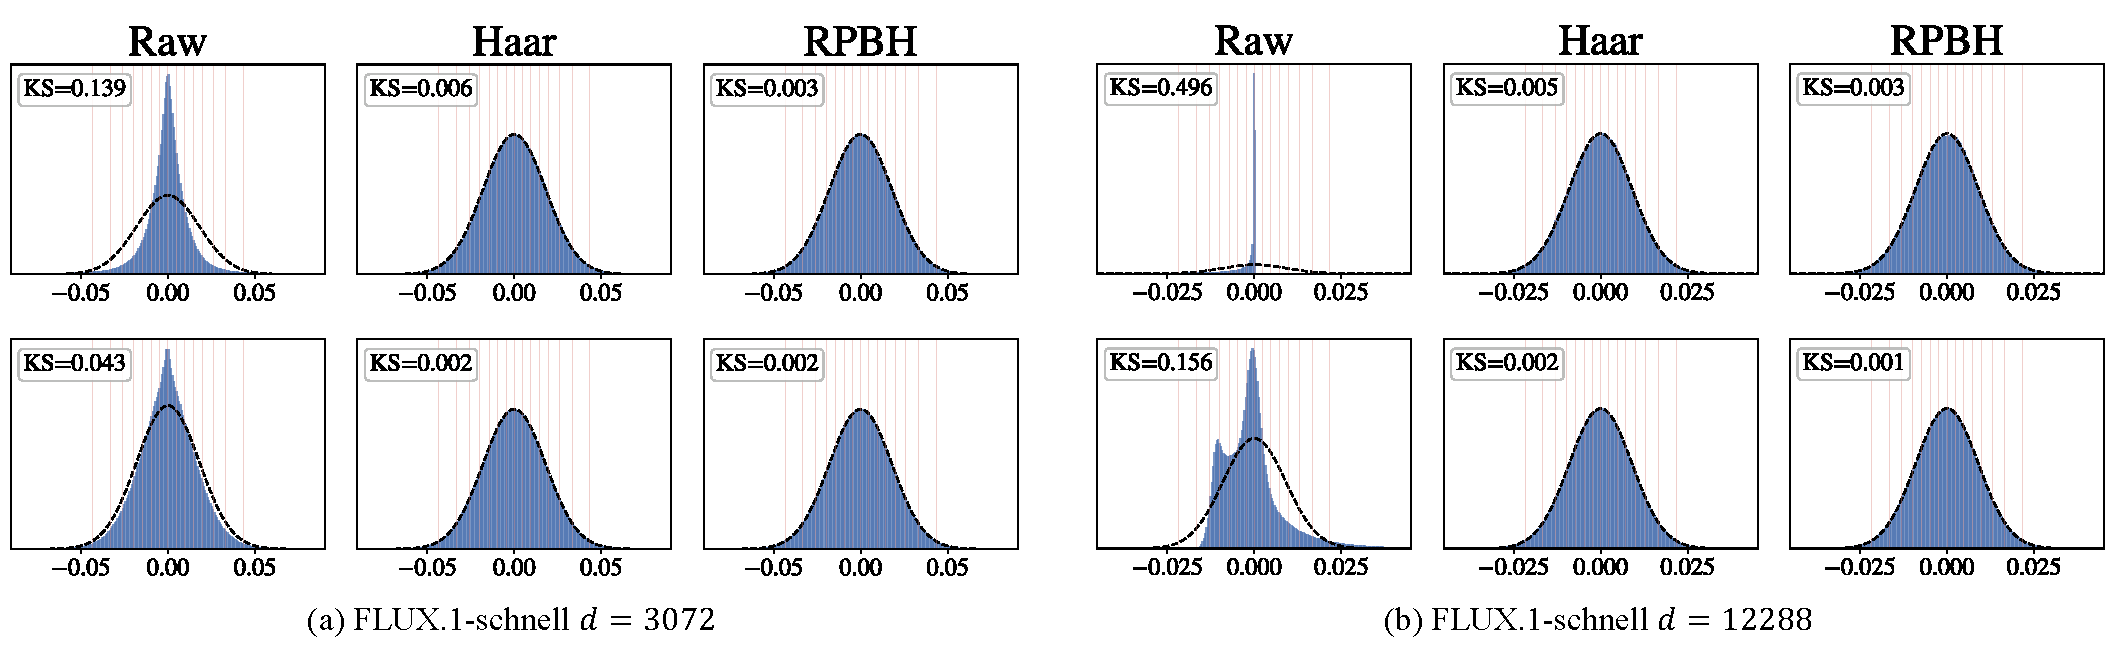
\includegraphics[width=\linewidth]{figures/rpbh_beta.pdf}
\vspace{-8mm}
\caption{Rotated activation coordinates follow the dimension marginal $f_d$. For (a) an attention projection ($d{=}3072$) and (b) a feed-forward projection ($d{=}12288$) of FLUX.1-schnell, each cell plots the distribution of activation tokens with no rotation (Raw), a dense Haar rotation, and the RPBH. The dashed curve is the target $\mathcal{N}(0,1/d)$ and the inset reports the Kolmogorov--Smirnov distance to it. The light red vertical ticks mark the bin edges of the shared Lloyd--Max $W4$ codebook, which is fit to $f_d$ and reused for both weights and activations.}
\vspace{-4mm}
\label{fig:distribution}
\end{figure*}


\subsection{Randomized permuted block-Hadamard}
\label{sec:method:rpbh}
Quantizing all layers of dimension $d$ with one codebook built from $f_d$ works only if the rotated coordinates follow that marginal. A Haar rotation $\boldsymbol{\Phi}_d$ from~\cite{zandieh2025turboquant} makes them follow $f_d$ exactly. Since the rotation cancels in the matrix product for any orthogonal $\boldsymbol{\Pi}_d$, we are free to choose it for efficiency, as long as it keeps the marginal close to $f_d$. A dense Haar rotation costs $O(d^2)$ in both time per token and storage, which dominates the per-image activation cost. We instead realize $\boldsymbol{\Pi}_d$ as a randomized permuted block-Hadamard (RPBH) rotation~\cite{ailon2009fast, tropp2011improved},
\begin{equation}
\boldsymbol{\Pi}_d = \mathrm{blkdiag}(\mathbf{H}_h \mathbf{D}_1, \ldots, \mathbf{H}_h \mathbf{D}_{d/h}) \cdot \mathbf{P}_\pi,
\label{eq:rpbh}
\end{equation}
where $\mathrm{blkdiag}(\cdot)$ places its arguments as diagonal blocks, $\mathbf{H}_h$ is a $h \times h$ Walsh--Hadamard matrix, each $\mathbf{D}_i$ is a Rademacher sign diagonal, and $\mathbf{P}_\pi$ is the matrix of a uniform random permutation $\pi$ drawn once per dimension. It admits an $O(d \log h)$ transform through a permutation gather and a per-block Fast Walsh--Hadamard Transform, and stores as a sign vector and a permutation array rather than a $d \times d$ matrix. Unlike a full Randomized Hadamard Transform (RHT)~\cite{ashkboos2024quarot, tseng2024quip}, whose Walsh--Hadamard matrix exists only on power-of-two dimensions, the block form is constructible on any $d$. In practice, $h$ is the largest power of two dividing $d$, giving $h \in \{128, 512, 1024, 2048, 4096\}$ across all evaluated models.

The leading permutation $\mathbf{P}_\pi$ acts first and keeps the marginal close to $f_d$ at low bit-width. Without it, each block-Hadamard mixes only within its block, and an outlier concentrated in one block never spreads across the others. $\mathbf{P}_\pi$ spreads coordinates across blocks, so every block receives a balanced share of the input mass with high probability over $\pi$. Crucially, this permutation need not be data-dependent. Prior quantizers calibrate it by outlier magnitude~\cite{lin2024duquant}, column importance~\cite{gu2026lopro}, or per-block mass~\cite{sanjeet2026pushing}. RPBH instead draws it uniformly at random, which suffices for any input as the following proposition shows.


\begin{proposition}[Universal variance concentration]
\label{prop:marginal}
Let $\boldsymbol{\Pi}_d$ be the RPBH rotation of Equation~\eqref{eq:rpbh} on $d = kh$ with $k$ blocks of size $h$, and $\tilde{\mathbf{x}}$ a fixed unit vector with $\mu_\infty = \|\tilde{\mathbf{x}}\|_\infty^2$. For every $\delta \in (0, 1)$, with probability at least $1 - \delta$ over $\boldsymbol{\Pi}_d$, every coordinate $z_i$ of $\boldsymbol{\Pi}_d \tilde{\mathbf{x}}$ is centered with
\begin{equation}
\mathrm{Var}(z_i \mid \pi) \in \Big[\tfrac{1-\rho}{d},\; \tfrac{1+\rho}{d}\Big], \qquad \rho = d\,\mu_\infty \sqrt{\tfrac{1}{2h}\log\tfrac{4k}{\delta}}.
\label{eq:prop-var}
\end{equation}
\end{proposition}

Since $\rho$ stays small unless one coordinate carries an outsized share of the norm, the variance bound of Equation~\eqref{eq:prop-var} keeps the marginal of $\boldsymbol{\Pi}_d \tilde{\mathbf{x}}$ close to $\mathcal{N}(0, 1/d)$ and the Lloyd--Max codebook near-optimal. We prove the proposition in the supplementary material~\ref{sec:supp-proof-srht}. Section~\ref{sec:ablation:rotation} confirms that removing the permutation degrades low-bit robustness.


% The leading permutation $\mathbf{P}_\pi$ acts first and is what keeps the marginal close to $f_d$ at low bit-width. Without it, each block-Hadamard mixes only within its block, so an outlier concentrated in one block, a common pattern for DiT activation channels, is never spread across blocks and the marginal depends on how the input aligns with the blocks. $\mathbf{P}_\pi$ redistributes coordinates across blocks first, so by a balls-and-bins argument every block receives a balanced share of the input mass with high probability over $\pi$.


% \begin{proposition}[Universal marginal matching]
% \label{prop:marginal}
% Let $\boldsymbol{\Pi}_d$ be the SRHT of Equation~\eqref{eq:srht} on $d = kb$ and $\tilde{\mathbf{x}}$ a fixed unit vector with $\mu_\infty = \|\tilde{\mathbf{x}}\|_\infty^2$. For every $\delta \in (0, 1)$, with probability at least $1 - \delta$ over $\boldsymbol{\Pi}_d$, every coordinate $z_i$ of $\boldsymbol{\Pi}_d \tilde{\mathbf{x}}$ is centered with
% \begin{equation}
% \mathrm{Var}(z_i) \in \Big[\tfrac{1-\rho}{d},\; \tfrac{1+\rho}{d}\Big], \qquad \rho = d\,\mu_\infty \sqrt{\tfrac{1}{2b}\log\tfrac{2k}{\delta}}.
% \label{eq:prop-var}
% \end{equation}
% \end{proposition}

% Since $\rho$ stays small unless one coordinate carries an outsized share of the norm, the variance bound of Equation~\eqref{eq:prop-var} keeps the marginal of $\boldsymbol{\Pi}_d \tilde{\mathbf{x}}$ close to $\mathcal{N}(0, 1/d)$ and the Lloyd--Max codebook of Section~\ref{sec:prelim:turboquant} near-optimal. The permutation is what makes this hold for every input, since without it a contiguous block of outlier channels keeps its mass and inflates that block's variance, which the codebook cannot absorb at low bit-width. We prove the proposition in the supplementary material.

% Rotation-based LLM quantizers~\cite{chee2023quip, ashkboos2024quarot, liu2025spinquant} build cross-coordinate mixing into the rotation itself, with a full Walsh--Hadamard on power-of-two dimensions, a Kronecker product with a smaller Hadamard-admitting factor otherwise, or a learned orthogonal matrix, so they need no separate permutation. The Kronecker route needs a library of small Hadamard matrices and mixes coordinates only within a fixed grid. OrbitQuant instead keeps a purely block-diagonal Hadamard on power-of-two blocks and lets the leading permutation supply the cross-block mixing, a cheap coordinate shuffle that also yields the input-universal variance bound of Proposition~\ref{prop:marginal}. Section~\ref{sec:ablation:rotation} confirms that removing the permutation degrades low-bit robustness.


\subsection{Data-agnostic Codebook}
\label{sec:method:codebook}
Prior PTQ methods recalibrate because the activation range shifts with the timestep and prompt. OrbitQuant removes this dependence at the source. By Proposition~\ref{prop:marginal}, every coordinate of a normalized, RPBH-rotated activation stays close to the same marginal $f_d$, fixed by the dimension $d$ alone. We therefore run Lloyd--Max on $f_d$ offline to obtain a single codebook $\mathcal{C}_d$ per dimension, and quantizing reduces to normalizing, rotating, and mapping each coordinate to its nearest centroid, with no input statistics collected. One $\mathcal{C}_d$ serves every timestep, prompt, layer, and the weight rows of dimension $d$, which is what makes OrbitQuant calibration-free.

This codebook follows TurboQuant~\cite{zandieh2025turboquant}, which quantizes randomly rotated vectors against a fixed Beta-marginal codebook computed once. TurboQuant is a standalone vector quantizer for KV-cache and vector-database compression. It uses a dense $O(d^2)$ Haar rotation and operates as a quantize-dequantize codec, reconstructing each vector before use. OrbitQuant instead pairs the codebook with the structured RPBH rotation and absorbs it into the weights. The quantized operands then feed each linear layer directly, with no reconstruction and only a forward rotation at inference.
% it uses a dense $O(d^2)$ Haar rotation and rotates back on dequantization to reconstruct each vector. OrbitQuant instead pairs the codebook with the structured RPBH rotation and absorbs it into the weights, so weight-activation quantization needs only a forward rotation at inference and no inverse. 
Figure~\ref{fig:distribution} confirms the marginal matching at an attention projection ($d{=}3072$) and a feed-forward layer ($d{=}12288$). Raw activations deviate sharply from $f_d$, but after the RPBH rotation both weights and activations match $f_d \approx \mathcal{N}(0,1/d)$ as closely as a dense Haar rotation does, so a single codebook built from $f_d$ fits them all.

% A per-layer rotation would leave the $f_d$ marginal unchanged, so we share one $\boldsymbol{\Pi}_d$ across all layers of a dimension, which keeps the rotation setup small and can be fused into the preceding LayerNorm or AdaLN affine.




% \subsection{Shared rotation per input dimension}
% \label{sec:method:shared}

% TurboQuant draws a fresh rotation inside every quantizer instance. Two design choices in our setting motivate a different scope. First, in a DiT every linear layer with input dimension $d$ sees activations whose anisotropy structure is similar after layer normalization, so a per-layer rotation increases memory by $O(L \cdot d^2)$ for $L$ layers without measurably improving the marginal distribution. Second, fixing a single $\Pi_d$ across layers is a prerequisite for fusing the rotation into the preceding LayerNorm or AdaLN affine in a follow-up kernel. We therefore adopt a single rotation $\Pi_d$ per input dimension $d \in \mathcal{D}$, shared by every $(W, x) \in \mathcal{L}$ with that input dimension. A per-layer comparison is reported in  the supplementary material.

% \paragraph{Implementation.}
% We realize Equations~(\ref{eq:activation-rotate})--(\ref{eq:activation-quant}) as a PyTorch \texttt{forward\_pre\_hook} on each target \texttt{nn.Linear}. The hook returns $\hat{x}'$ as the modified input, and the layer's native forward then computes $\hat{W}' \hat{x}'$. A naive scalar quantizer would compute $|\tilde{x}_k - c_j|$ for every $(k, j)$ pair, requiring an $(N, d, 2^{b_a})$ intermediate tensor and exhausting GPU memory at $b_a \geq 6$. Because the codebook boundaries are sorted by construction, we instead use \texttt{torch.bucketize} for $O(\log L)$ binary search per coordinate. Further hook-architecture and caching details are in the supplementary.

% \subsection{Forward identity and rotation cancellation}
% \label{sec:method:cancel}

% Substituting Equations~(\ref{eq:rotated-weight}) and~(\ref{eq:activation-rotate}) into the linear-layer forward map yields
% \begin{equation}
% W' x' = W \Pi_d^\top \Pi_d \, x = W x,
% \label{eq:cancel}
% \end{equation}
% because $\Pi_d^\top \Pi_d = I_d$. When $\hat{W}'$ replaces $W'$ in the model and the pre-hook replaces $x'$ by $\hat{x}'$, the layer computes $\hat{W}' \hat{x}'$, a quantized estimate of $Wx$ with no inverse rotation needed at runtime. The rotated basis is the only basis ever materialized after the offline step in Equation~(\ref{eq:weight-quant}). The original-basis weight $W$ is overwritten and never re-instantiated.

% \paragraph{Error bound.}
% Writing $W' = \hat{W}' + E_w$ and $x' = \hat{x}' + e_x$, the output error decomposes as
% \begin{equation}
% W x - \hat{W}' \hat{x}' = E_w \hat{x}' + \hat{W}' e_x + E_w e_x.
% \label{eq:error}
% \end{equation}
% By the centroid condition of the Lloyd--Max quantizer applied row-wise in Equations~(\ref{eq:weight-quant}) and~(\ref{eq:activation-quant}), $e_x$ and each row of $E_w$ have expectation zero conditional on the magnitudes, with per-coordinate variance bounded by the Lloyd--Max distortion against $f_d$. The shared rotation $\Pi_d$ makes both row and activation errors isotropic in the rotated frame, so the cross terms in Equation~(\ref{eq:error}) average down across the matrix product.

% \subsection{SRHT and the leading permutation}
% \label{sec:method:srht}

% Equations~(\ref{eq:rotated-weight})--(\ref{eq:cancel}) hold for any orthogonal $\Pi_d$, but the codebook compatibility used in Equation~(\ref{eq:weight-quant}) depends on one structural property: $\Pi_d$ must produce an \emph{incoherent} representation of every unit-norm row of $W$ and every unit-norm activation, in the sense that the empirical marginal of $\Pi_d \tilde{x}$ matches $\mathcal{N}(0, 1/d)$ closely enough for the Lloyd--Max codebook of Section~\ref{sec:prelim:turboquant} to remain near-optimal.

% \paragraph{Why not dense Haar.}
% The Haar construction of Section~\ref{sec:prelim:turboquant} produces the exact marginal $f_d$, but at $O(d^2)$ cost per matrix-vector product and $O(d^2)$ memory for the rotation matrix. For the largest input dimension we encounter ($d = 12288$ on FLUX feed-forward down-projections), this is approximately 604\,MB in FP32, which must be held on CPU and copied on demand. The matrix-vector cost dominates the activation hook latency.

% \paragraph{SRHT construction.}
% OrbitQuant instead uses the canonical Subsampled Randomized Hadamard Transform~\cite{halko2011, tropp2011}:
% \begin{equation}
% \Pi_d = \mathrm{blkdiag}(H_b D_1, \ldots, H_b D_{d/b}) \cdot P_\pi,
% \label{eq:srht}
% \end{equation}
% where $H_b \in \{\pm 1/\sqrt{b}\}^{b \times b}$ is the Walsh--Hadamard matrix (Sylvester construction, $b$ a power of two), each $D_i$ is an independent $\pm 1$ diagonal with i.i.d.\ Rademacher signs, and $P_\pi$ is a uniform random permutation matrix on $d$ coordinates, drawn once per dimension and shared across all layers. For non-power-of-two $d$ we take $b$ to be the largest power of two dividing $d$. SRHT is orthogonal and admits an $O(d \log b)$ matrix-vector product via a permutation gather followed by a Fast Walsh--Hadamard Transform per block. For $d = 12288$ and $b = 4096$, this is roughly $2000\times$ cheaper than the dense Haar matmul, and the rotation buffer collapses from 604\,MB to one $b$-element sign vector per block plus a $d$-entry integer permutation array.

% \paragraph{Why the permutation matters.}
% Without $P_\pi$, the block-diagonal Hadamard acts only inside each block. Any structured outlier whose support is concentrated in a single block, a common pattern for activation channels in DiTs, is mixed within that block but never spread across blocks. The incoherence bound then depends on the input's block alignment, which the quantization hook cannot control. The permutation $P_\pi$ uniformly redistributes coordinates across blocks first: by a balls-and-bins argument, $\|P_\pi \tilde{x}\|_2^2$ allocates mass $\|\tilde{x}\|_2^2 / (d/b)$ to each block up to $O(\sqrt{\log d / b})$ fluctuation, with high probability over $\pi$. The block-Hadamard then sees a balanced input on every block, removing the alignment dependence.

% \begin{proposition}[SRHT universal incoherence]
% \label{prop:srht}
% Let $\Pi_d$ be the SRHT of Equation~(\ref{eq:srht}) with block size $b$ on dimension $d = kb$. For every fixed unit vector $\tilde{x} \in \mathbb{R}^d$ and every $\delta \in (0, 1)$,
% \begin{equation}
% \Pr\!\left[\|\Pi_d \tilde{x}\|_\infty > \sqrt{\frac{2 \log(2d/\delta)}{b}}\right] \leq \delta,
% \label{eq:incoherence}
% \end{equation}
% where the probability is taken over the joint draw of the permutation $\pi$ and the block signs $\{D_i\}$.
% \end{proposition}

% The proof follows the standard SRHT concentration argument and is given in the supplementary material. For our smallest block size ($b = 1024$ on FLUX $d = 3072$), Proposition~\ref{prop:srht} with $\delta = 10^{-3}$ bounds $\|\Pi_d \tilde{x}\|_\infty$ by $\sqrt{2 \log(6 \cdot 10^6) / 1024} \approx 0.16$, uniformly over $\tilde{x}$. Combined with the per-coordinate variance $1/d$, the marginal $\Pi_d \tilde{x}$ matches $\mathcal{N}(0, 1/d)$ up to a $1 + O(\log b / b)$ multiplicative factor in MSE distortion. This justifies reusing the Lloyd--Max codebook of Section~\ref{sec:prelim:turboquant} under both Haar and SRHT rotations.

% \paragraph{Contrast with rotation-based LLM PTQ.}
% QuIP~\cite{quip2024}, QuaRot~\cite{quarot2024}, and SpinQuant~\cite{spinquant2024} also rotate before quantization, but they target LLMs with power-of-two hidden dimensions and no AdaLN. The rotation is fused with attention rather than absorbed into stored weights, and the input distribution into the rotation is already pre-mixed by upstream attention or Kronecker structure. The leading permutation of Equation~(\ref{eq:srht}) is therefore unnecessary in their setting, and block-RHT alone suffices. In a DiT, raw post-norm activations enter the quantization hook without any upstream cross-block mixing, so the explicit permutation is the missing piece. Section~\ref{sec:ablation} verifies that removing it degrades low-bit robustness.
